\chapter{Introduction}
\label{chap:intro}
\vspace{-1cm}


\lsection{Motivation. The problem of odor localization}

The use of new technologies based on artificial noses for the detection and classification of odor sources has the potential to be a true game-changer in many fields \cite{stitzel2011artificial, wilson2009applications}. Tasks such as security monitoring for the detection of high-risk substances/gases in residential and industrial environments, food quality control assessment \cite{DymerskiChmiel11}, environmental protection and field measurement, biometric identification \cite{RodriguezLujan2013279}, medical control \cite{YanezToledano12}, noninvasive routine monitoring, etc, are all taking benefit from the improvements of these techniques.
Moreover, the combination of modern machine olfaction technologies with mobile robotics allows to implement new target identification algorithms that can tackle not only detection tasks \cite{vazquez2013integracion} but higher level odor-related search and monitoring tasks as well \cite{Hu2013, Marjovi2011, marjovi2010olfactory, song2011olfaction, jatmiko2011robots, Marques2006, Hayes02distributedodor}.

While simulated environments are often successfully used to demonstrate the performance of generic search tasks \cite{Mcgill2011,HayesMG01}, the chaotic nature of gases and odor plumes often create a poor balance between the accuracy and computational requirements of the models \cite{Torney2009}.
Most odorants have latency and decay, which turn out to be complex temporal structures that are difficult to model.
This is why it is so important to step out of simulations and have a way to actually test odor search algorithms in the real world \cite{Hu2013, Marjovi2013, song2011olfaction, HayesMG03}.
Also, the uncertainty inherent to the problem of odor localization seems to make possible a drastic reduction in the completion time by parallelizing the search with more than a single agent \cite{Hu2013, Marjovi2013, Marjovi2011, Hayes02distributedodor, HayesMG01}. Here is where the cooperation among robots comes into play, as it is possible to implement a wide range of collaborative search algorithms that include centralized, de-centralized and distributed approaches \cite{Hu2013, Mcgill2011, marjovi2010olfactory}.


Thus, the main motivation and goal of this work is to provide the scientific community with an open robotic platform that simplifies the process of implementing and testing such kind of odor search algorithms.
The developed robots will incorporate artificial noses by design, and the high-level control system will allow to use them efficiently as a active odor-sensing networks.
Novel bio-inspiration for collaborative strategies could finally provide efficient solutions to odor search tasks \cite{Mcgill2011, Reynolds2013, Dunbabin2012, raey10, KongcunM09, arleo07}, and these types of platforms are needed in order to accelerate their incorporation and fulfillment of necessities in industry and in other aspects of the society.


\lsection{State of the art. Odor detection and robotics}

This project has its base in previous work developed at \emph{Grupo de Neurocomputaci\'{o}n Biol\'{o}gica} in \emph{Universidad Aut\'{o}noma de Madrid}. An electronic nose module called ``Olus2'' (Fig. \ref{fig:introduction/OlusAndTGS2600}), created by David Y\'{a}\~{n}ez from Deutecno\footnote{\url{http://www.deutecno.com/}}, has already been used to evaluate various odor detection and classification tasks \cite{YanezToledano12, Yanez09}.
The Olus2 module has also been integrated with a modular robot in a project by Tom\'{a}s V\'{a}zquez Rubio \cite{vazquez2013integracion}, to demonstrate response upon odor perception of a snake-shaped robot. Also, the ongoing work at the group by Alejandro Peque\~{n}o Zurro -who is currently addressing the single-robot odor localization task- has provided to be an enriching collaboration towards a better characterization the odor sensor response.

%Tin odor sensors. How do they work?
The sensing element of most artificial noses is usually a semiconductor based on \emph{tin dioxide} ($SnO_2$).
With the adequate manufacturing technique it is possible to create tin dioxide based materials that present conductivity variations in the presence of a gas.
Those variations in conductivity are measured to be proportional to the perceived concentrations of gas, so the sensor can be effectively modeled as a resistor that varies with odor intensity. Though, the transient responses of tin oxide sensors are usually very pronounced and can make the concentration-measurement task non-trivial.
Also, the semiconductor material needs to be heated up in order to have odor sensitivity, so these kind of sensors usually include a resistive heating element.
Tin dioxide gas sensors are often used in breath analyzers and smoke alarms due to their good sensitivity to organic compounds like ethanol and carbon monoxide \cite{wilson2009applications, stitzel2011artificial}.
A strongly recommended lecture to understand the underlying principles and inner working of these types of sensors is ``Nanostructured Tin Dioxide Materials for Gas Sensor Applications'' by T.A. Miller et al. \cite{MillerBakrania06nanostructured}.

\begin{figure}[h!]
\centerline{\mbox{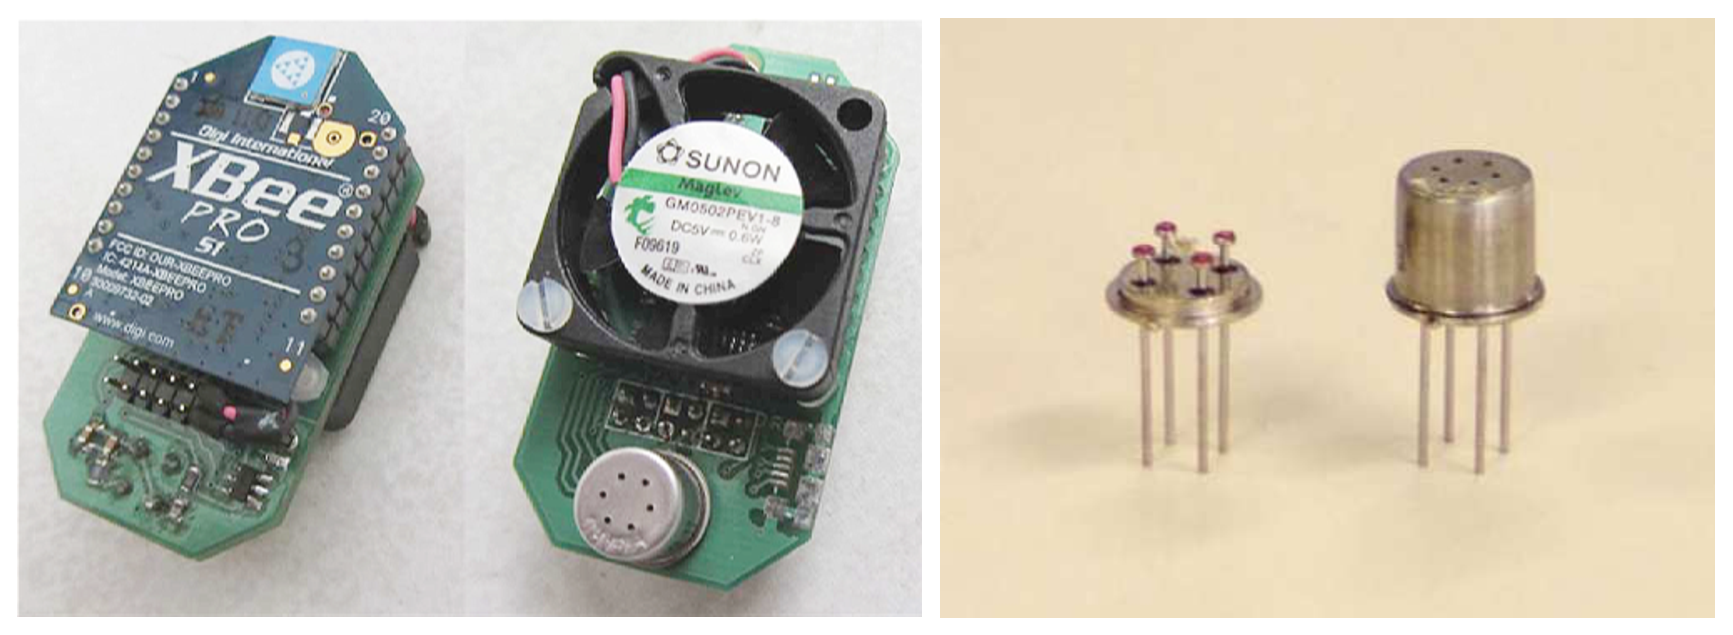
\includegraphics[width=15cm]{images/introduction/OlusAndTGS2600.eps}}}
\captionFigure{Olus2 artificial nose module and odor sensor detail}
{fig:introduction/OlusAndTGS2600}{
Olus2 modules (left) incorporate the TGS2600 odor sensor (right), which is based on tin dioxide semiconductor. Sources: \cite{vazquez2013integracion} and \url{http://figaro.com/}}
\end{figure}

%Odor source modeling
Whilst gas-sensor technology has becomed quite advanced in the last years \cite{pearce2003handbook}, there is still no ideal solution to be found, and the detection of odors has to rely on quite uncertain and noisy responses.
Even with a noisy sensory input, the odor search problem would be trivial to solve if odor concentrations were gradients that varied monotonically according to distance - but that is not the case. The random nature of odor plumes adds up into the equation and the complexity of the problem increases dramatically \cite{Torney2009}.
There is also variability in the types of odor sources that can be used as targets. As the molecular structure of scent particles provides each odorant with different fading times, it is not only needed to model the effective detection area of the odor plume but also its latency and evolution over time \cite{Mcgill2011}.


%Multimodal sensor integration
Having a good model of the target is then a crucial part towards the localization of odors, but those models must account for the uncertainty in the odor sensor response. These imprecisions, inherent to gas sensing, can be tackled with the particularly interesting approach that is multimodal sensor integration \cite{Hein24072012, song2011olfaction, arleo07}. The incorporation of other types of input from devices like video cameras, proximity sensors or air flow directivity sensors, can contribute to remove noise and increase the precision of odor plume detections \cite{Marjovi2013, Hayes02distributedodor}.
In the cases where the odor sources are not disperse but very localized instead, it can be possible to use a simple threshold model and obtain reasonable results \cite{vazquez2013integracion, acosta2013diseno}.




The other critical factor towards an efficient solution to the odor search task is the selection of a sensible search strategy. Search algorithms have been extensively studied for many decades, and the most popular approaches can be classified in three main groups: gradient-based algorithms (i.e. hill climbing \cite{Mcgill2011}), probabilistic methods (i.e. environment mapping \cite{FoxKo05}, bayesian, kalman or particle filters \cite{jatmiko2011robots}), and biologically inspired algorithms (i.e. biased random walks \cite{Hein24072012} or chaotic search \cite{KongcunM09}).
Gradient-based algorithms can be susceptible to local maxima and they depend on the monotonic variation of measurements, which as has been discussed is not the case for odor plumes. Probabilistic search methods and mapping, while requiring high computational resources and memory, are often the preferred approach when the environment is fully characterized.
Bio-inspired search algorithms, on the other hand, come into play when there is uncertainty within the definition of a search problem (i.e. when the search area is not well defined or odor sources may appear and disappear with different latencies).
All of these algorithms can be applied to single-agent tasks and to multi-robot search as well.


%\cite{Mcgill2011} % REVIEW General solutions to search of multiple emission sources
% The lack of a common set of validation cases and reference algorithms that form a ground truth for comparative analysis makes it impossible to directly compare the different algorithms and weigh their merits for different applications. This begs the questions of what should such a reference set involve and how should comparative analysis be performed. Some obvious characteristics are clearly relevant from the literature and evident in Table I: the initial distribution of sources and robots, the presence of obstacles, background flow, dead space (involving no perceptible gradient) and occluded sources, the level of disparity between source strengths, and the time-varying nature of source injection and removal.
% Gradient-based algorithms (i.e. hill climbing), which can be susceptible to local maxima.
% Probabilistic methods (i.e. mapping and bayesian, Kalman or particle filtering), which usually require high computational power
% Biologically inspired algorithms: biased random walks

%\cite{FoxKo05} % A Hierarchical Bayesian Approach to the Revisiting Problem in Mobile Robot Map Building





\subsection{Cooperative search strategies}

\vspace{-0.3cm}

Recent studies have shown that odor search algorithms that involve the collaboration among multiple robots can lead to a more efficient odor search \cite{Hu2013, Mcgill2011, marjovi2010olfactory}.
This project sets its focus on these approaches while leaving open the possibility of implementing single-robot strategies, as they can be considered the particular case of a \emph{N-robot} system where $N=1$.
Inter-robot cooperation can be implemented in various forms: an optimization of the available energy resources (i.e. live decision of which robot performs a surveillance task), by sharing mapping information \cite{Marjovi2011}, with the minimization of unnecessary redundancy during search, etc.
This kind of cooperativity among robots is covered by Appendix \ref{Appendix:designStrategies}.

Other types of collaboration can include multimodal sensory feedback as seen in some animal species. An interesting example of this approach is well reflected with an implementation where a robot would generate acoustic signals upon odor detection, and thus allow others reach the target much faster \cite{song2011olfaction}.
Supervised search where robots cooperate with humans to enhance the performance of a given search task \cite{GoodrichPendleton11, KonoligeOrtiz04}, can also be considered a form of multimodal sensory feedback.
Human-robot interaction already plays a crucial role in gas detection for environmental monitoring \cite{Dunbabin2012} as well as in search and rescue of targets \cite{Hu2013}.
Autonomous robot team management has also received inspiration from human behavior, for instance with the incorporation of dynamical team and sub-team creation \cite{BradshawFeltovich09} that leads to improvements in human-agent-robot interaction.

%\cite{Marjovi2011} % cooperative search in structured environments. robot communication (mapping)

%\cite{Hu2013} % cooperative search review, hybrid simulations

%\cite{song2011olfaction} % odor plume search real robots. multimodal sensors. one robot locates the odor and emmits a sound to attract other robots to the odor source

%----Human interaction in search

%\cite{Dunbabin2012} % Robots for Environmental Monitoring: Significant Advancements and Applications

%\cite{BradshawFeltovich09} % human-like team creation and management. joint activity coordination and cooperation with human entities. human-agent-robot teams. dinamical creation of teams and subteams

%\cite{GoodrichPendleton11} % human interaction with bio-inspired robot teams

%\cite{KonoligeOrtiz04} % Centibots: Very Large Scale Distributed Robotic Teams. human interaction. integrated end-to-end system


%----Emerging group-level intelligence through simple local interaction

Higher levels of cooperation can also be achieved without the need of a global deterministic specification of the search algorithms. Bio-inspired strategies that are based on \emph{swarm robotics} take advantage on the group-level intelligence that can emerge from simple local interactions, a subject with raising interest among the odor-locating research community \cite{Torney2009}.
Some experiments have already demonstrated the capability of a robot swarm to transverse an odor plume by the means of simple inter-robot interaction with soft-defined rules \cite{Marjovi2013}.
An example of these rules can be lightweight agent-avoidance routines that lead to a global exploratory behavior \cite{Marques2006}.
The behavioral rules can also be context-dependent. For instance, long-range exploration could be inhibited when local odors are detected or when energy resources are running low.

%\cite{Marjovi2013} % odor plume modeling and simulation, evaluation with real robots (roomba w/ laptops). swarm robotic formation (equally spaced, transversal line)

%\cite{Torney2009} % the task becomes highly nontrivial due to the generation of heterogeneous, dynamically changing filamental concentrations that do not decrease monotonically with distance to the source.
% odor search. emerging group-level intelligence. local interaction->emerging behavior

%\cite{Marques2006} % efficient local searching behaviours. By default, the agents tend to avoid each other, leading to the emergence of exploration behaviours when no chemical cue exists in the neighbourhood

\vspace{-0.5cm}
\subsubsection{Biased L\'{e}vy-walk search}
\vspace{-0.3cm}
%----Biased random search
While classical heuristic solutions could be adequate for the localization of odorants that have a fixed position and invariant properties, these are not an option for problems with uncertainty (i.e. a brute-force search algorithm would not be efficient for monitoring an area that is weakly defined).
On the other hand, bio-inspired strategies that do not rely on prior system assumptions could finally provide efficient solutions to the odor search task \cite{Hein24072012, Mcgill2011, raey10, arleo07}.
\emph{Random walks} or chaotic search have generally been the preferred source of inspiration for their robustness and performance within a reasonable simplicity \cite{KongcunM09}.
\emph{L\'{e}vy flights} are a specific type of random walk that can be commonly observed in nature \cite{Reynolds2013}.


\begin{figure}[h!]
\centerline{\mbox{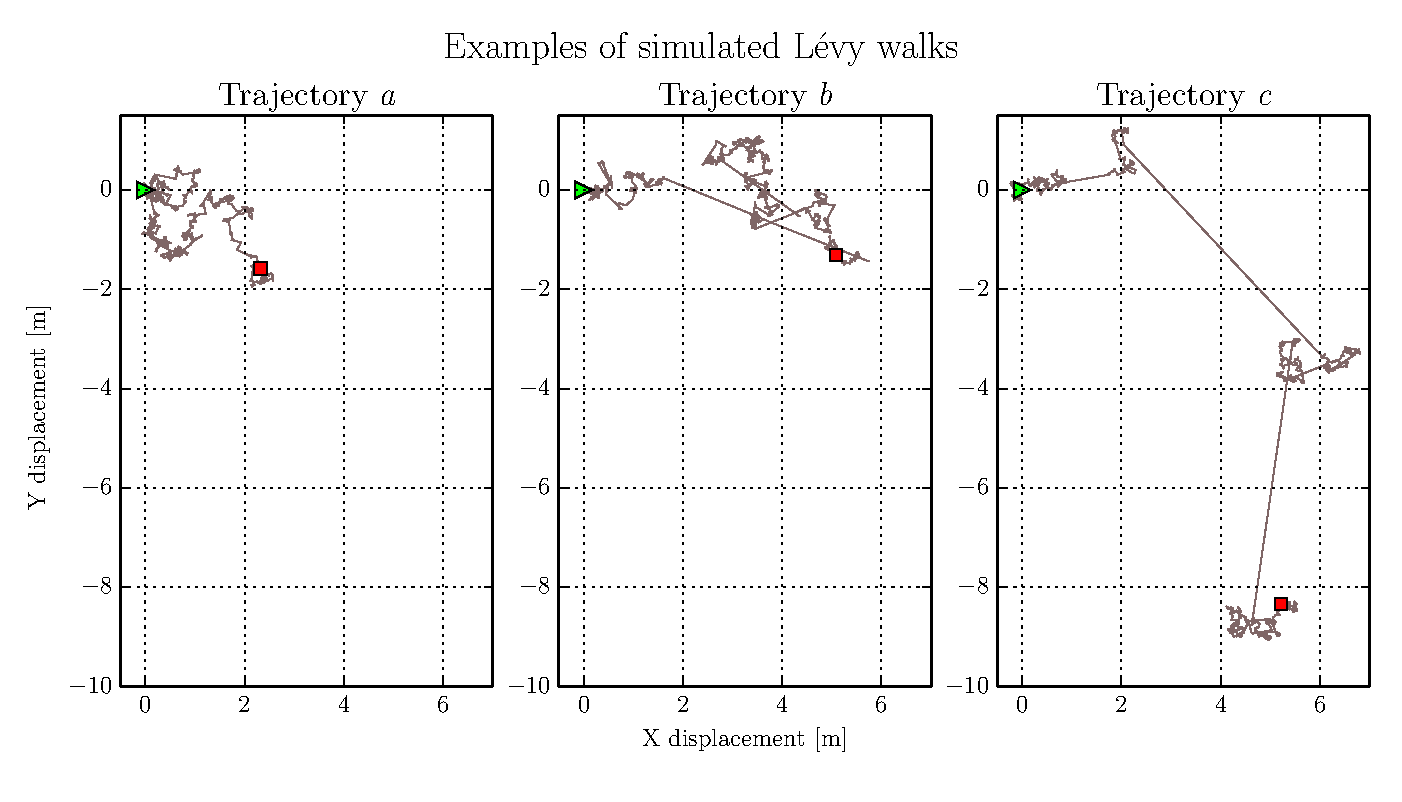
\includegraphics[width=15cm]{images/introduction/simulated_levy_walks.eps}}}
\captionFigure{Examples of simulated 2-dimensional L\'{e}vy walks}
{fig:introduction/simulated_levy_walks}{
2000 iterations of three different simulations that show various random walks based on a L\'{e}vy probabilistic distribution. The starting and ending points are marked in green and red respectively. Changes in the stability parameter $\alpha$ cause differences in the exploratory behavior: larger values generate a more localized search \emph{(a)}, while decreasing $\alpha$ can have the effect of a faster-growing expansion (\emph{b} and \emph{c}). The angular direction has a uniform distribution, but could also be nuanced in order to modulate the L\'{e}vy search strategy.
}
\end{figure}


They are formed by variable length steps that combine clusters of short-sized moves with more distant travel paths (see Fig. \ref{fig:introduction/simulated_levy_walks}). This variation in the length of the steps is determined by a L\'{e}vy probabilistic distribution that is heavy-tailed, which leads to a random occurrence of longer steps.
Species like honeybees, ants, marine predators, and even human hunters have shown the successful use of these L\'{e}vy patterns for search \cite{Raichlen23122013}.
As the behavior of animals and insects does not rely solely on random distributions, it can be possible to increase the eficiency by biasing the parameters of random navigation in real time with multimodal sensory input integration \cite{arleo07}. It has been shown that even the incorporation of feedback from a noisy sensor response can lead to a reduction in search times \cite{Hein24072012, KongcunM09}.

%\cite{arleo07} % multimodal sensory integration. navigation strategies. bio-inspiration

%\cite{raey10} % bio-inspiration for navigation strategies

%\cite{KongcunM09} % An Improved Artificial Fish Swarm Algorithm Based on Chaotic Search and Feedback Strategy. Clustering, optimization

%\cite{Hein24072012} % Sensing and decision-making in random search. multi-modal sensor integration. a lack of signal is not a lack of information. Searchers that receive no signal can quickly abandon target-poor regions. On the other hand, receiving a strong signal leads a searcher to concentrate search effort near targets. results show that including even a simple response to noisy sensory data can dominate other features of random search, resulting in lower mean search times


%----L\'{e}vy walks (Fig. \ref{fig:introduction/simulated_levy_walks})

%\cite{Reynolds2013} % levy walk model formulation % http://iopscience.iop.org/0295-5075/102/1/18001/article/
% Effective leadership in animal groups when no individual has pertinent information about resource locations: How interactions between leaders and followers can result in L\'{e}vy walk movement patterns

%\cite{Raichlen23122013} % evidence of levy walk in human hunters




The performance of many of these types of novel bio-inspired search strategies has yet to be evaluated for the odor search task. Whilst it is common to use simulators, it has already been discussed that the randomness of odorant plumes makes their modeling computationally inefficient. Hybrid simulators could be a solution for this issue, since they can combine the precision of actual odor source measurements with the performance obtained with off-line algorithm optimization \cite{HayesMG03}. Though, all these implementations would still need to step out of theoretical calculations towards the actual implementation and validation with robots in the real world.


%\cite{HayesMG01} % odor search. distributed algorithm. demonstrate group robots transverse odor plume. faithful simulator

%\cite{HayesMG03} % Off-line optimization and validation with real robots. einforcement learning algorithm to optimize performance across group size, showing that it can be useful not only for improving real world odor localization, but also for quantitatively characterizing the influence of group size on task performance


\vspace{-0.5cm}
\subsection{Existing robotic platforms}
%Open-source 3D-printable platforms

The need for real-world validation of odor search tasks raises the question of what are the available robotic platforms that can be used.
Among the requirements that can be specified are: the presence of odor sensors, a localization system to register the position of the robots over time, a well-dimensioned power source, and a reduced cost. Also, the ability to easily incorporate other multimodal sensor information is essential \cite{Hayes02distributedodor}, but is a feature commonly lacking in odor search implementations.
Another important requirement is the size of the robots, as they should be small in order to minimize unnecessary odor plume disturbances.
Most of the previous work that can be found on literature demonstrating implementations of odor search strategies have relied on platforms such as the \emph{iRobot}\footnote{\url{http://www.irobot.com/}} \cite{Marjovi2013, marjovi2010olfactory} or other proprietary solutions \cite{ElfwingDoya14, jatmiko2011robots, KonoligeOrtiz04, HayesMG03}. Those robots are lacking either a reduced size or a simple expandability, which can cause difficulties towards standardization of real-world odor search implementations.


\emph{Printbots} are open-source robotic platforms that can be 3D-printed \cite{GonzalezValero11miniskybot,ValeroGonzalez12creativity,Garcia-Saura2012,ValeroGonzalezOOML12}, and they could provide the low-cost expandability and repeatability that are needed for these multi-robot implementations. As they are open, Printbots can be evolved by the community and thus easily modified to incorporate the improvements made in any part of the world. This means, for instance, that a wind sensor integration made for a particular odor location study could be rapidly merged back into the original robot design, and thus make the replication and further evolution of the experiment conveniently accessible to other researchers.

%\cite{jatmiko2011robots} % Robots implementation for odor source localization using PSO algorithm. odor localization, real robots, 12 ceiling cameras

%\cite{KonoligeOrtiz04} % Centibots: Very Large Scale Distributed Robotic Teams. human interaction. integrated end-to-end system

%\cite{acosta2013diseno} % simula fuente de olor con una luz, usa placa beaglebone, open-loop motor control

%\cite{Hayes02distributedodor} % conducting polymer-based odor sensors possess the combination of speed and sensitivity necessary to enable real world odor plume tracing. simple local position, odor, and flow information, tightly coupled with robot behavior, is sufficient

%\cite{Marjovi2013} % odor plume modeling and simulation, evaluation with real robots (roomba w/ laptops). swarm robotic formation (equally spaced, transversal line)

%\cite{marjovi2010olfactory} % cooperative odor search, real robots, wireless network for robot localization










\vspace{-0.3cm}
\subsubsection{Spatial localization techniques}
\vspace{-0.3cm}
%Trabajo previo de tracking. GPS, Cámaras, etc

A good perception of the position of robot agents in their environment is necessary for some search algorithms. Most importantly, robot localization is needed at a experimental level in order to evaluate the performance of search strategies \cite{jatmiko2011robots, Fox00Pro}.
The field of automated robot tracking has been widely studied for many years, and a number of robust solutions have appeared \cite{Gut02Exp}. Whilst GPS (\emph{Global Positioning System}) is the preferred approach for outdoor environment, it only provides accuracy at the meter range and higher accuracies are needed for local or indoor search \cite{ChenSun10}.
The combination of GPS with other radio-frequency-based approaches (i.e. position inference based on GSM or Wi-Fi signal strength \cite{Ferris06gaussianprocesses}) can provide more resolution at the expense of a cost that does not scale for large robot swarms.
The cost of robot localization can be minimized with the use of more simple sensors, as it is possible to obtain accuracy from
devices that have noisy measurements
with the use of state-of-the-art technologies like artificial intelligence algorithms \cite{Thrun98landmark, FoxKo05}.

Landmark-based localization techniques (such as the use of beacons) are one of the most extended methods, as they can be applied to most types of input \cite{EscaleraMoreno96, Fox00Pro}. Most of the robot localization approaches for indoor environments are vision-based \cite{chen2009towards}. Some decide to place markers in the environment and mount cameras on board each robot \cite{gifford2009low, HongboHongnian07} while others place markers in the robots and then use external cameras to inform each robot of its position \cite{reina2012zeppelin, jatmiko2011robots}. This last alternative can be the most attractive for experimental research environments, since it provides a low cost solution and the added convenience of having the experiments recorded in video.




%\cite{Thrun98landmark} % Bayesian Landmark Learning for Mobile Robot Localization

%\cite{FoxKo05} % A Hierarchical Bayesian Approach to the Revisiting Problem in Mobile Robot Map Building


%\cite{EscaleraMoreno96} % Continuous mobile robot localization by using structured light and a geometric map



%\cite{Fox00Pro} % A Probabilistic Approach to Collaborative Multi-Robot Localization. cameras and laser rangefinders



%\cite{chen2009towards} % Towards multi-robot formations: study on vision-based localization system

%\cite{jatmiko2011robots} % Robots implementation for odor source localization using PSO algorithm. odor localization, real robots, 12 ceiling cameras

%\cite{reina2012zeppelin} % zePPeLIN: Ceiling camera networks for the distributed path planning of ground robots

%\cite{HongboHongnian07} % Ceiling Light Landmarks Based Localization and Motion Control for a Mobile Robot

%\cite{gifford2009low} % Low-Cost Mobile Robot Localization Using Only a Downward-Facing Webcam. OJO VA EN EL ROBOT



%\cite{Ferris06gaussianprocesses} % Gaussian Processes for Signal Strength-Based Location Estimation

%\cite{Gut02Exp} % An Experimental Comparison of Localization Methods Continued

%\cite{ChenSun10} % Localization for Multirobot Formations in Indoor Environment





\vspace{-0.5cm}
\lsection{Project approach, methodology and goals}

The high variability in the parameter definition of odor search problems (\emph{i.e. initial distribution of robots in the search area, presence of obstacles, amount of odor sources and their latency, etc.}) has caused the absence of a standardized method for directly validating nor comparing the performance of each search algorithm \cite{Mcgill2011}.
Part of the problem arises from the use of proprietary robotic platforms in previous studies, which are expensive and not suitable for more than a few algorithm implementations. The standardization around a robotic platform should then be of help towards a common base of comparison for odor search algorithms.

This project will try to address the issue, with the design of an open-source set of tools to allow the future implementation and field testing of a broad range of search algorithms with a set of low-cost replicateable robots.

The specific goals are:

\vspace{-0.5cm}

\begin{packed_enum}
	\item Design of a 3D printed structure for the mobile robots. It must be easy to replicate the robot to create a swarm of low-cost identical agents.
	\item Layout of the electronic boards, it is a requisite that they are energy efficient, have multi-sensor integration (an active artificial nose, battery monitoring, and also temperature, humidity and distance sensors), and based on Arduino.
	\item Selection of the technique for localizing the robots in the search space.
	\item Design and implementation of the bi-directional communication method that allows simple access to the experiment data in real time, with an abstraction layer in Python to allow high-level programming of the robots.
	\item Implementation of a closed-loop robot controller based on way points.
	\item Validation of the robot platform for odor detection.
	\item Assembly of at least three robots equipped with artificial noses.
	\item Open-source publication of the platform.
\end{packed_enum}

\vspace{0.0001cm}







\subsection{Relation with the Degree in ITST}
Being a multidisciplinar project, the required technical knowledge has been covered by most of the courses of the Degree in Telecommunication Technology and Service Engineering (ITST) at Universidad Aut\'{o}noma de Madrid.
Some specific courses from the itinerary on \emph{Design and Implementation of Electronic Communication Systems} have resulted of special interest (\emph{Sistemas de Control}, \emph{Sistemas Electr\'{o}nicos Digitales}, \emph{Instrumentaci\'{o}n y Medida}, \emph{Tecnolog\'{i}a Electr\'{o}nica de Sistemas}), and the core subjects have also received complementary education in the fields of electronics (\emph{Tecnolog\'{i}a de dispositivos}, \emph{Circuitos electr\'{o}nicos digitales}, \emph{Circuitos anal\'{o}gicos y de potencia}, \emph{Fundamentos de microprocesadores}), software and signal processing (\emph{Programaci\'{o}n I y II}, \emph{Sistemas lineales}, \emph{Teor\'{i}a de la comunicaci\'{o}n}, \emph{Tratamiento digital de se\~{n}ales}, \emph{Aritm\'{e}tica para el procesamiento de se\~{n}al}), as well as real-time networking (\emph{Redes I y II}, \emph{Redes Multimedia}).





\singlespacing
\subsection{Overview and milestones of the project}
\begin{enumerate}
	\item \textbf{Documentation and literature research (state of the art)}
	\item \textbf{\emph{GNBot} robotic platform design}
	\begin{enumerate}
		\item Printed mechanical structure
		\begin{enumerate}
			\item Design of the 3D parts (chassis, wheels, electronic board and battery supports, etc.)
			\item Motor type selection (two continuous rotation servomotors)
			\item Power requirement analysis and battery selection (two 9V rechargeable batteries)
		\end{enumerate}
		\item Electronic elements
		\begin{enumerate}
			\item Design of a PCB for the multi-sensor integration (including polarization circuits for the odor sensor, battery level monitor, luminosity sensors, IR range finders, an electronic compass, and the temperature and humidity sensor)
			\item Industrial manufacture of the designed circuit boards (20 unit order to \url{http://www.seeedstudio.com/})
		\end{enumerate}
		\item Software and communication interface
		\begin{enumerate}
			\item Development of the low-level control routines for Arduino
			\item Development of the ZigBee-based wireless communication protocol
			\item Development of the abstraction layer with Python
		\end{enumerate}
	\end{enumerate}
	\item \textbf{Assembly, testing and experiments}
	\begin{enumerate}
		\item Assembly and test of the prototype GNBot
		\item Implementation of a light landmark based localization system (documented in Appendix \ref{Appendix:lightLandmarks}).
		\item Design of the vision-based automatic robot tracking software (OpenCV and Python), adapted to the developed visual markers to provide X-Y position and angle orientation feedback
		\item Battery duration and performance measurements
		\item Implementation of a closed-loop way-point navigation algorithm
		\item Fabrication of the low-profile odor sources, to be used as targets for the search
		\item Robot platform multimodal sensor range characterization
		\item Assembly and test of a swarm of four final-version GNBot robots
	\end{enumerate}
	\item \textbf{Publication, contest participation and documentation}
	\begin{enumerate}
		\item \textbf{Publication submission and acceptance to the \emph{Living Machines 2014} International conference}, and participation of the project in the \emph{Arquimedes National Research Contest}. See Appendix \ref{Appendix:circuits}
		\item Creation of a website and GitHub repository for the open-source publication of the developed GNBot platform
	\end{enumerate}
\end{enumerate}
\onehalfspacing

The lenght of the project has been 12 months, at a rate of 3 hours/day. With the open-source publication of the developed platform the author expects to have contributed towards an acceleration in the development of cooperative robotic odor localization strategies.

Website of the GNBot project:  \url{https://github.com/carlosgs/GNBot/}


\newpage \thispagestyle{empty} % Página vacía

